\documentclass[11pt]{article}
\usepackage[margin=1in]{geometry}
\usepackage{graphicx}
\usepackage{booktabs}
\usepackage{array}
\usepackage{enumitem}
\usepackage{caption}
\usepackage{float}

% Simple line for fill-in blanks
\newcommand{\fillin}{\rule{2.5em}{0.4pt}}

\title{MIPS Datapath Lab Report}
\author{Kaushik Vada}
\date{CS161 -- Lab 2 and Lab 3}

\begin{document}
\maketitle

\section{Type Decode Unit}


\begin{table}[H]
  \centering
  \caption{Opcode patterns for instruction types.}
  \begin{tabular}{lcccc}
    \toprule
    Input (opcode bit) & R-format & lw & sw & beq \\
    \midrule
    Op5 & 0 & 1 & 1 & 0 \\
    Op4 & 0 & 0 & 0 & 0 \\
    Op3 & 0 & 0 & 1 & 0 \\
    Op2 & 0 & 0 & 0 & 1 \\
    Op1 & 0 & 1 & 1 & 0 \\
    Op0 & 0 & 1 & 1 & 0 \\
    \bottomrule
  \end{tabular}
\end{table}

\begin{figure}[H]
  \centering
  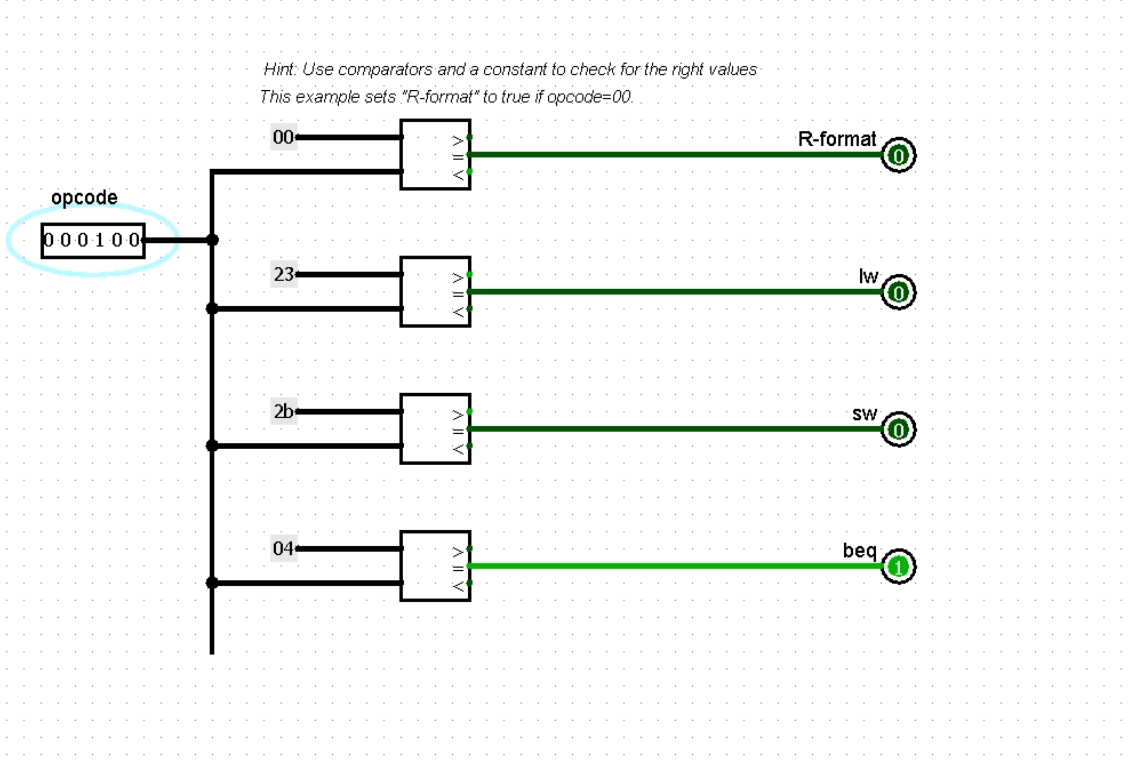
\includegraphics[width=0.9\linewidth]{Type_Decode_Unit.png}
  \caption{Type Decode unit after adding opcode comparators.}
\end{figure}

\section{Control Decode Truth Table}


\begin{table}[H]
  \centering
  \caption{Control-decode truth table.}
  \begin{tabular}{lcccc}
    \toprule
    Output & R-format & lw & sw & beq \\
    \midrule
    RegDst   & 1     & 0     & \textit{X} & \textit{X} \\
    ALUSrc   & 0     & 1     & 1          & 0 \\
    MemtoReg & 0     & 1     & \textit{X} & \textit{X} \\
    RegWrite & 1     & 1     & 0          & 0 \\
    MemRead  & 0     & 1     & 0          & 0 \\
    MemWrite & 0     & 0     & 1          & 0 \\
    Branch   & 0     & 0     & 0          & 1 \\
    ALUOp1   & 1     & 0     & 0          & 0 \\
    ALUOp0   & 0     & 0     & 0          & 1 \\
    \bottomrule
  \end{tabular}
\end{table}

\section{Control Decode Implementation}


\begin{figure}[H]
  \centering
  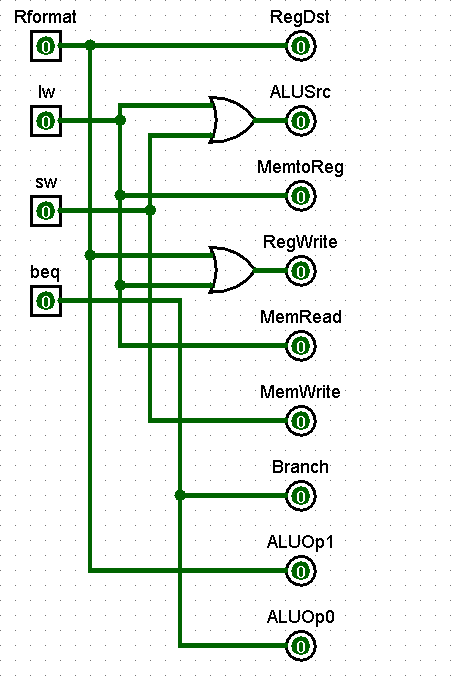
\includegraphics[width=0.9\linewidth]{Control_Decode_circuit.png}
  \caption{Control Decode unit with all outputs wired.}
\end{figure}

\section{Control Logic Wiring}


\begin{figure}[H]
  \centering
  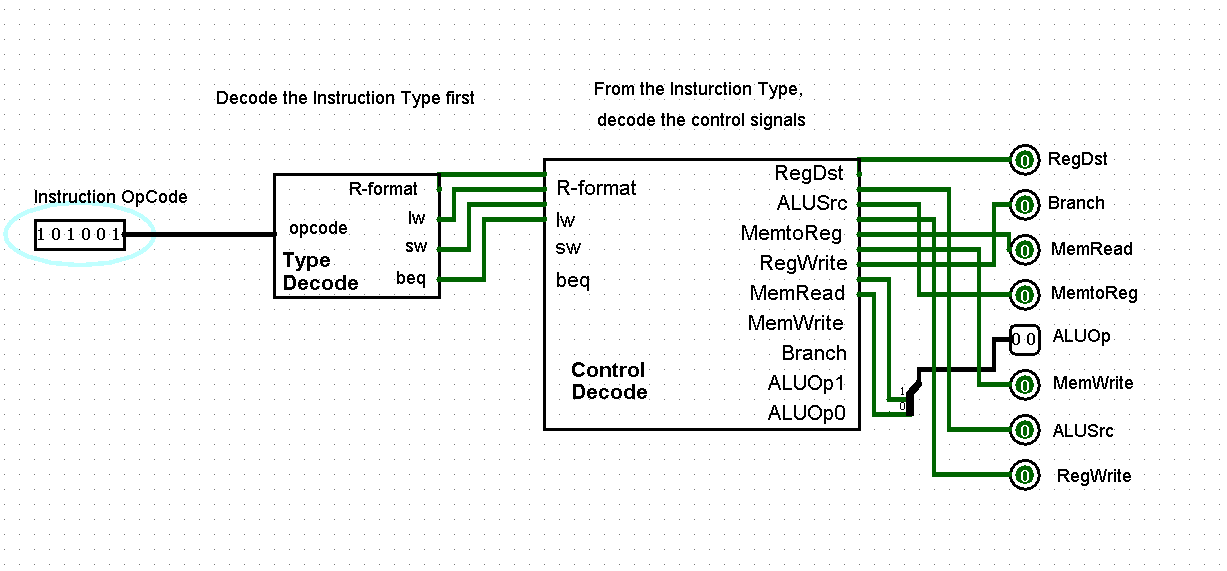
\includegraphics[width=0.9\linewidth]{wired_Control_block.png}
  \caption{Completed control logic wiring.}
\end{figure}

\section{ALU Control Unit}


\begin{table}[H]
  \centering
  \caption{ALU control mapping.}
  \begin{tabular}{ccccccccc}
    \toprule
    ALUOp1 & ALUOp0 & F5 & F4 & F3 & F2 & F1 & F0 & Operation \\
    \midrule
    0 & 0 & X & X & X & X & X & X & 0010 \\
    0 & 1 & X & X & X & X & X & X & 0110 \\
    1 & 0 & X & X & 0 & 0 & 0 & 0 & 0010 \\
    1 & 0 & X & X & 0 & 0 & 1 & 0 & 0110 \\
    1 & 0 & X & X & 0 & 1 & 0 & 0 & 0000 \\
    1 & 0 & X & X & 0 & 1 & 0 & 1 & 0001 \\
    1 & 0 & X & X & 1 & 0 & 1 & 0 & 0111 \\
    \bottomrule
  \end{tabular}
\end{table}

\begin{figure}[H]
  \centering
  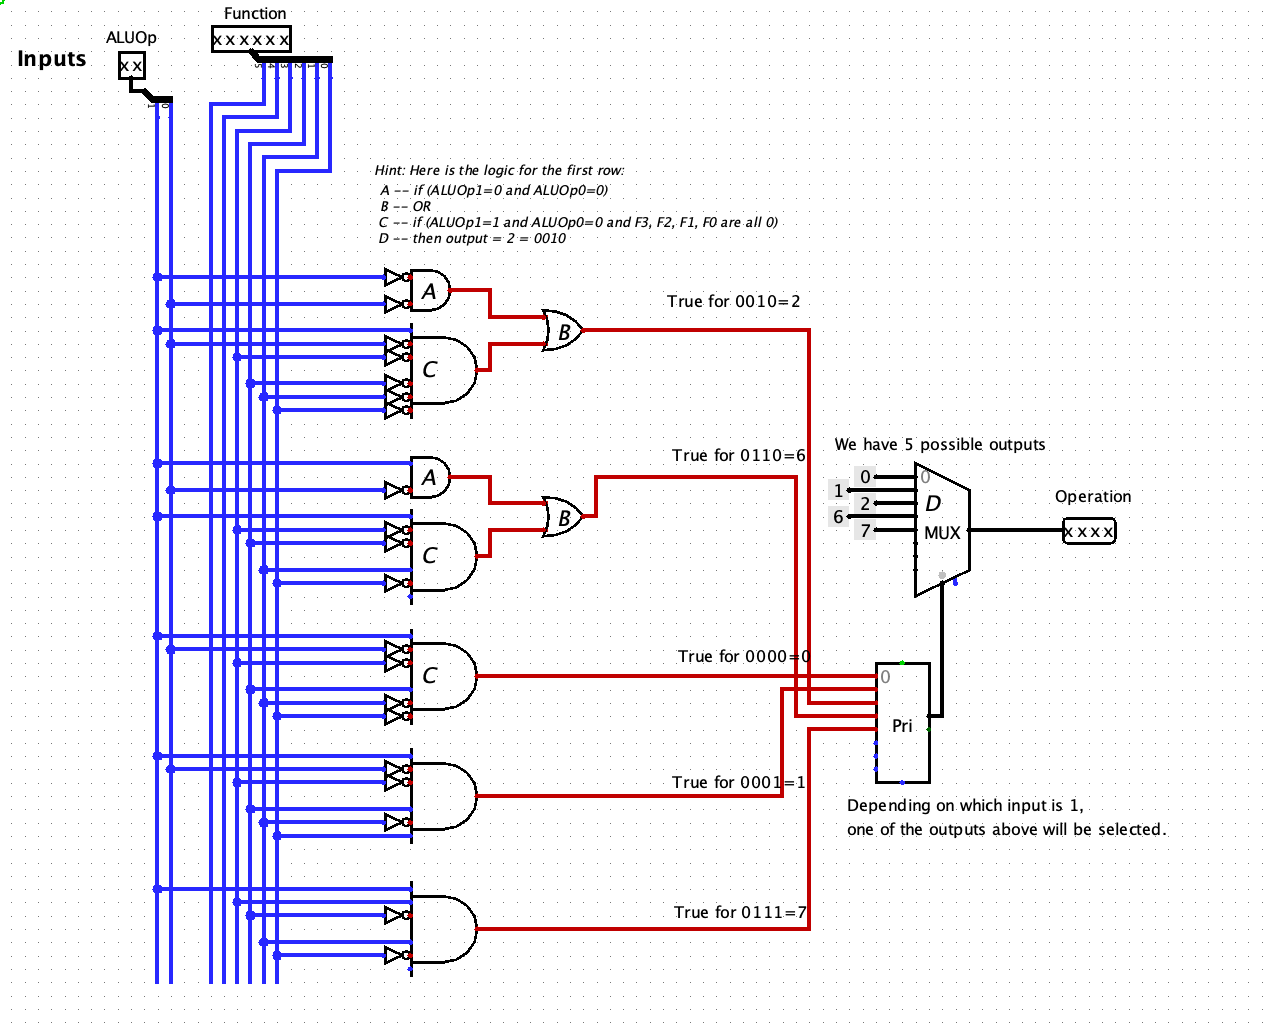
\includegraphics[width=0.9\linewidth]{ALU_Control_Circuit.png}
  \caption{ALU Control with priority encoder and mux logic filled in.}
\end{figure}

\section{Datapath Wiring}


\begin{figure}[H]
  \centering
  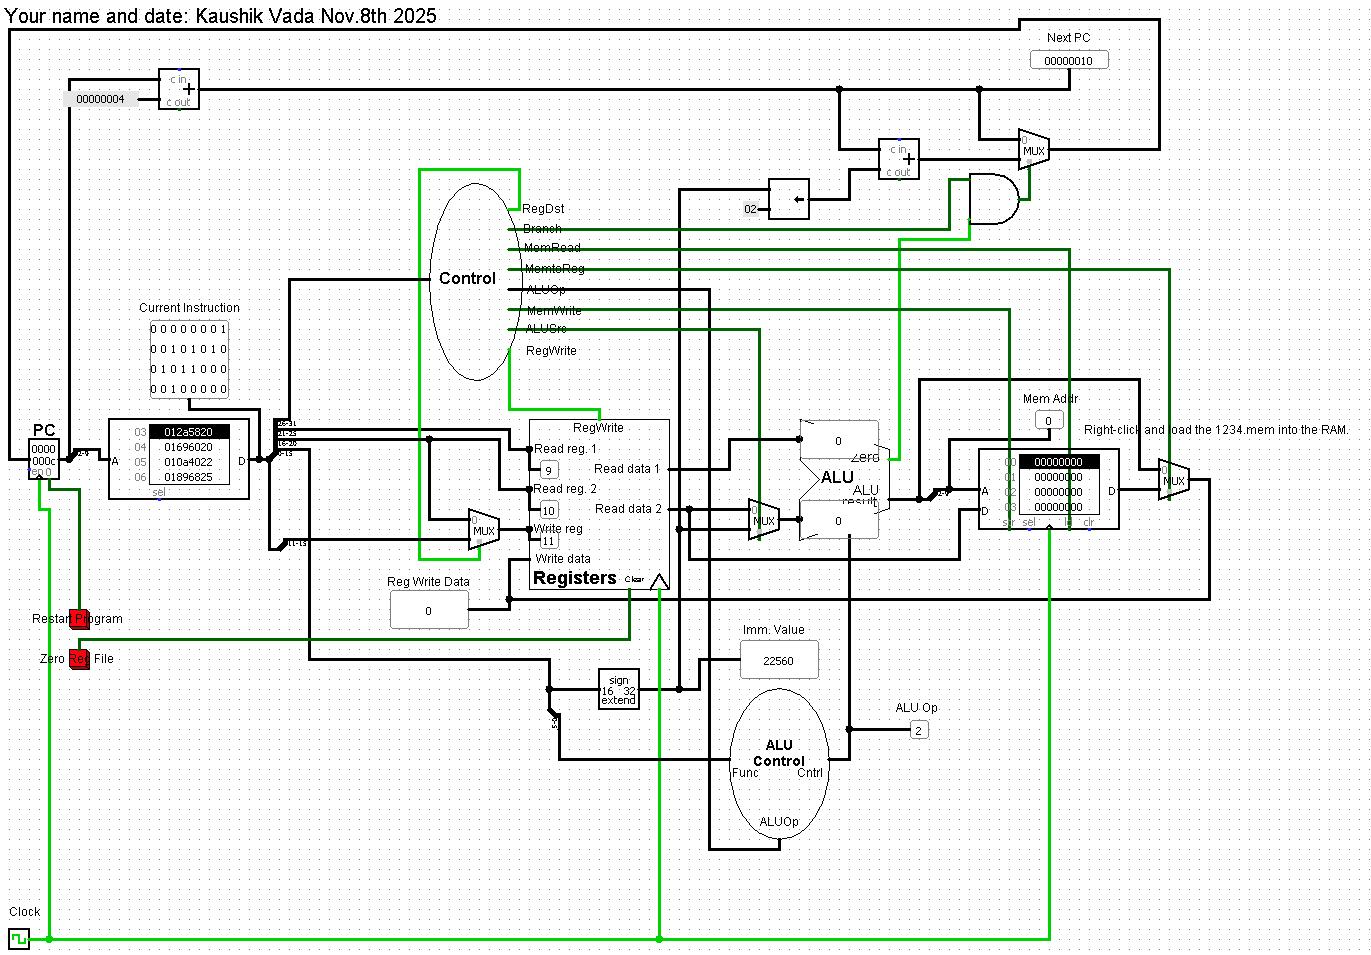
\includegraphics[width=0.9\linewidth]{fully_wired_datapath.png}
  \caption{Completed processor wiring (datapath view).}
\end{figure}

\newpage
\section{Program Execution Results}


\begin{table}[H]
  \centering
  \caption{Final register file contents to report.}
  \begin{tabular}{lccccccc}
    \toprule
    Register & $t0$ & $t1$ & $t2$ & $t3$ & $t4$ & $t5$ & $t6$ \\
    \midrule
    Value & 0 & 1 & 2 & 3 & 4 & 5 & 1 \\
    \bottomrule
  \end{tabular}
\end{table}




\end{document}
% .
